\section{Prototyp}
\label{sec:prototyp}
Unser Prototyp umfasst wie beschrieben drei Komponenten, den Web-Service, eine Smartphone- sowie eine Smartwatch-Anwendung. 

Entsprechend unserer definierten Anwendungsfälle (s. Kapitel \ref{sec:useCases}) kann man mit unserer Anwendung
\begin{itemize}
\item{die eigene Position auf einen Raum genau bestimmen,}
\item{Notizen in einem Raum anbringen und anzeigen,}
\item{Notizen mit Ereignissen verknüpfen und bei diesem zur Anzeige bringen und}
\item{angebrachte Notizen wieder löschen.} 
\end{itemize}


\subsection{Smartwatch}
Aufgrund der bereits beschriebenen Einschränkungen einer Smartwatch (s. Kap. \ref{sec:einschraenkungen}) haben wir uns im ersten Schritt die von Android-Wear bereitgestellten UI-Elemente intensiv angesehen. Unter den verschiedenen Möglichkeiten unsere gewünschten Notizen, bestehend aus Titel und Text, darzustellen, erschien uns die Darstellung in Form von Cards\footnote{Eine Übersicht der Android-Wear-UI-Patterns befindet sich unter \url{http://developer.android.com/design/wear/patterns.html}} am geeignetsten.

Um die Anzeige mehrerer Notizen auf dem kleinem Display der Smartwatch zu realisieren, haben wir uns überlegt die Cards horizontal in einer Art Liste anzuordnen. Eine solche Anordnung lässt sich als 2D-Picker\todo{einleitenden Text in Footnote? Wenn ja, dann bei allen Footnotes}\footnote{Eine Erklärung des 2D-Pickers befindet sich unter  \url{http://developer.android.com/training/wearables/ui/2d-picker.html}} mithilfe eines GridViewPagers realisieren. Des Weiteren lassen sich bestehende Notizen über einen Button löschen, der in Form eines Mülleimers dargestellt wird. 

Ursprünglich hatten wir geplant, dass es möglich sein sollte, eine Vermessung der Räume direkt über die Uhr durchzuführen. Den entsprechenden Dialog hatten wir als weitere Card umgesetzt, die über eine vertikale Wischgeste aufrufbar sein sollte. Das Problem war allerdings diese Funktionalität im Rahmen des 2D-Pickers
zu realisieren. Der 2D-Picker bildet immer ganze Matrizen ab, in der jede weitere Zeile gleich viele Elemente enthalten muss. In unserem Fall hätten wir dazu pro Notiz eine neue Einstellungscard instantiieren müssen. Mehrere Einstellungscards sähen nicht nur merkwürdig aus, sondern hätten auch Verwirrung gestiftet.\todo{Bild erzeugen und hierhin!} Des Weiteren haben wir festgestellt, dass es Usus ist, dass komplexere Dialoge im Wearable-Umfeld auf das Smartphone ausgelagert sind. Daher haben auch wir uns dazu entschieden, diese Funktionalität auf dem Smartphone zu implementieren.


Die Abbildungen \ref{fig:ScreenshotWatchEckig} und \ref{fig:ScreenshotWatchRund} zeigen
die Notizendarstellung unseres Prototyps. Die Smartwatch-Anwendung besteht aus der abgebildeten Ansicht, die ggf. mehrfach instantiiert wird.

\begin{figure}[H]
\centering
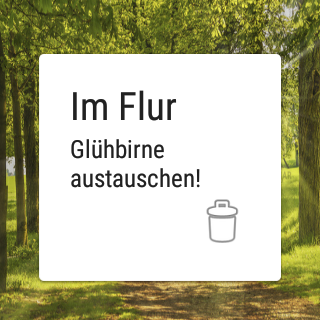
\includegraphics[width=0.3\linewidth]{../Bilder/ScreenshotWatchEckig}
\caption{Screenshot unserer Uhr mit eckigem Display}
\label{fig:ScreenshotWatchEckig}
\end{figure}

\begin{figure}[H]
\centering
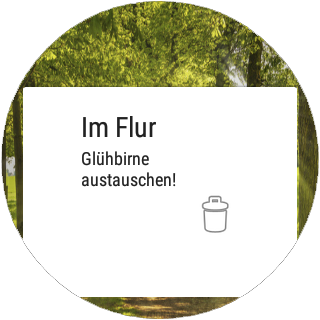
\includegraphics[width=0.3\linewidth]{../Bilder/ScreenshotWatchRund}
\caption{Screenshot unserer Uhr mit rundem Display}
\label{fig:ScreenshotWatchRund}
\end{figure}

\subsection{Smartphone}
Unsere Smartphone-Anwendung besteht aus zwei Ansichten. Die Hauptansicht erlaubt es Notizen zu erstellen und zur Smartwatch zu schicken (s. Abb. \ref{fig:ScreenshotPhoneMainActivity}), während eine weitere Ansicht zur Steuerung des Vermessungsvorgang (s. Abb. \ref{fig:ScreenshotPhoneRoomScanner}) dient.
 
\begin{figure}[H]
\centering
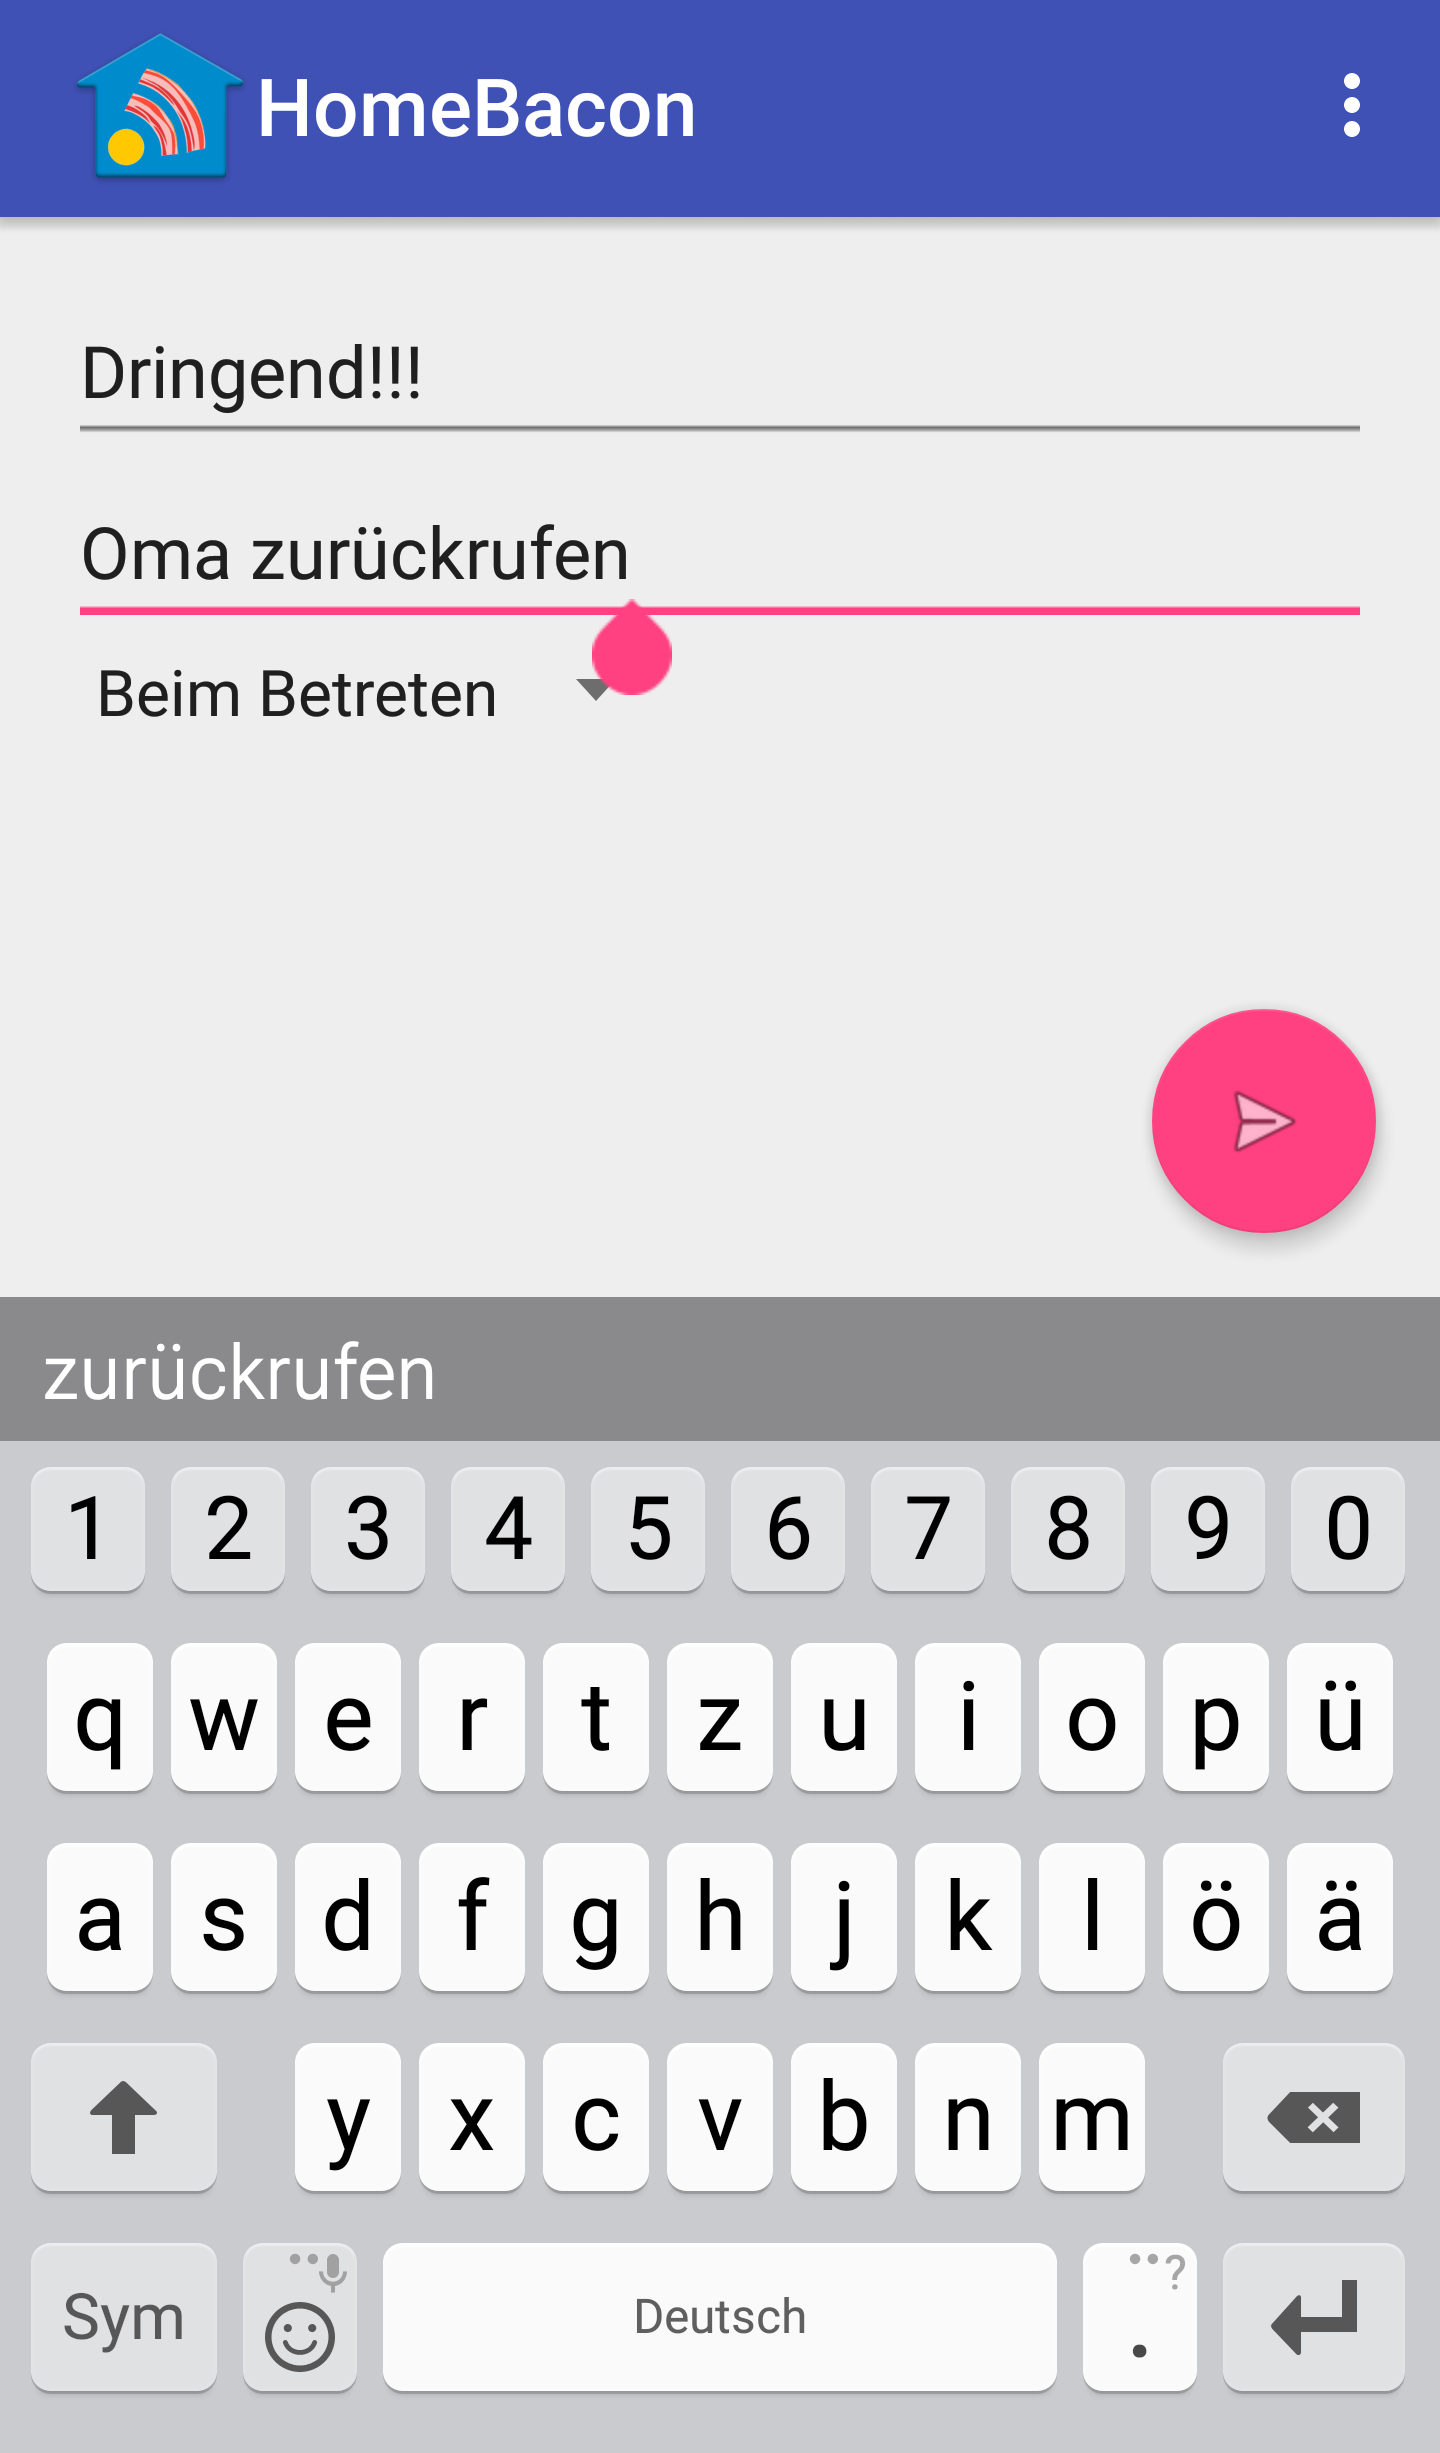
\includegraphics[width=0.4\linewidth]{../Bilder/ScreenshotPhoneMainActivity}
\caption{Screenshot der Ansicht zum Erstellen von Notizen}
\label{fig:ScreenshotPhoneMainActivity}
\end{figure}

\begin{figure}[H]
\centering
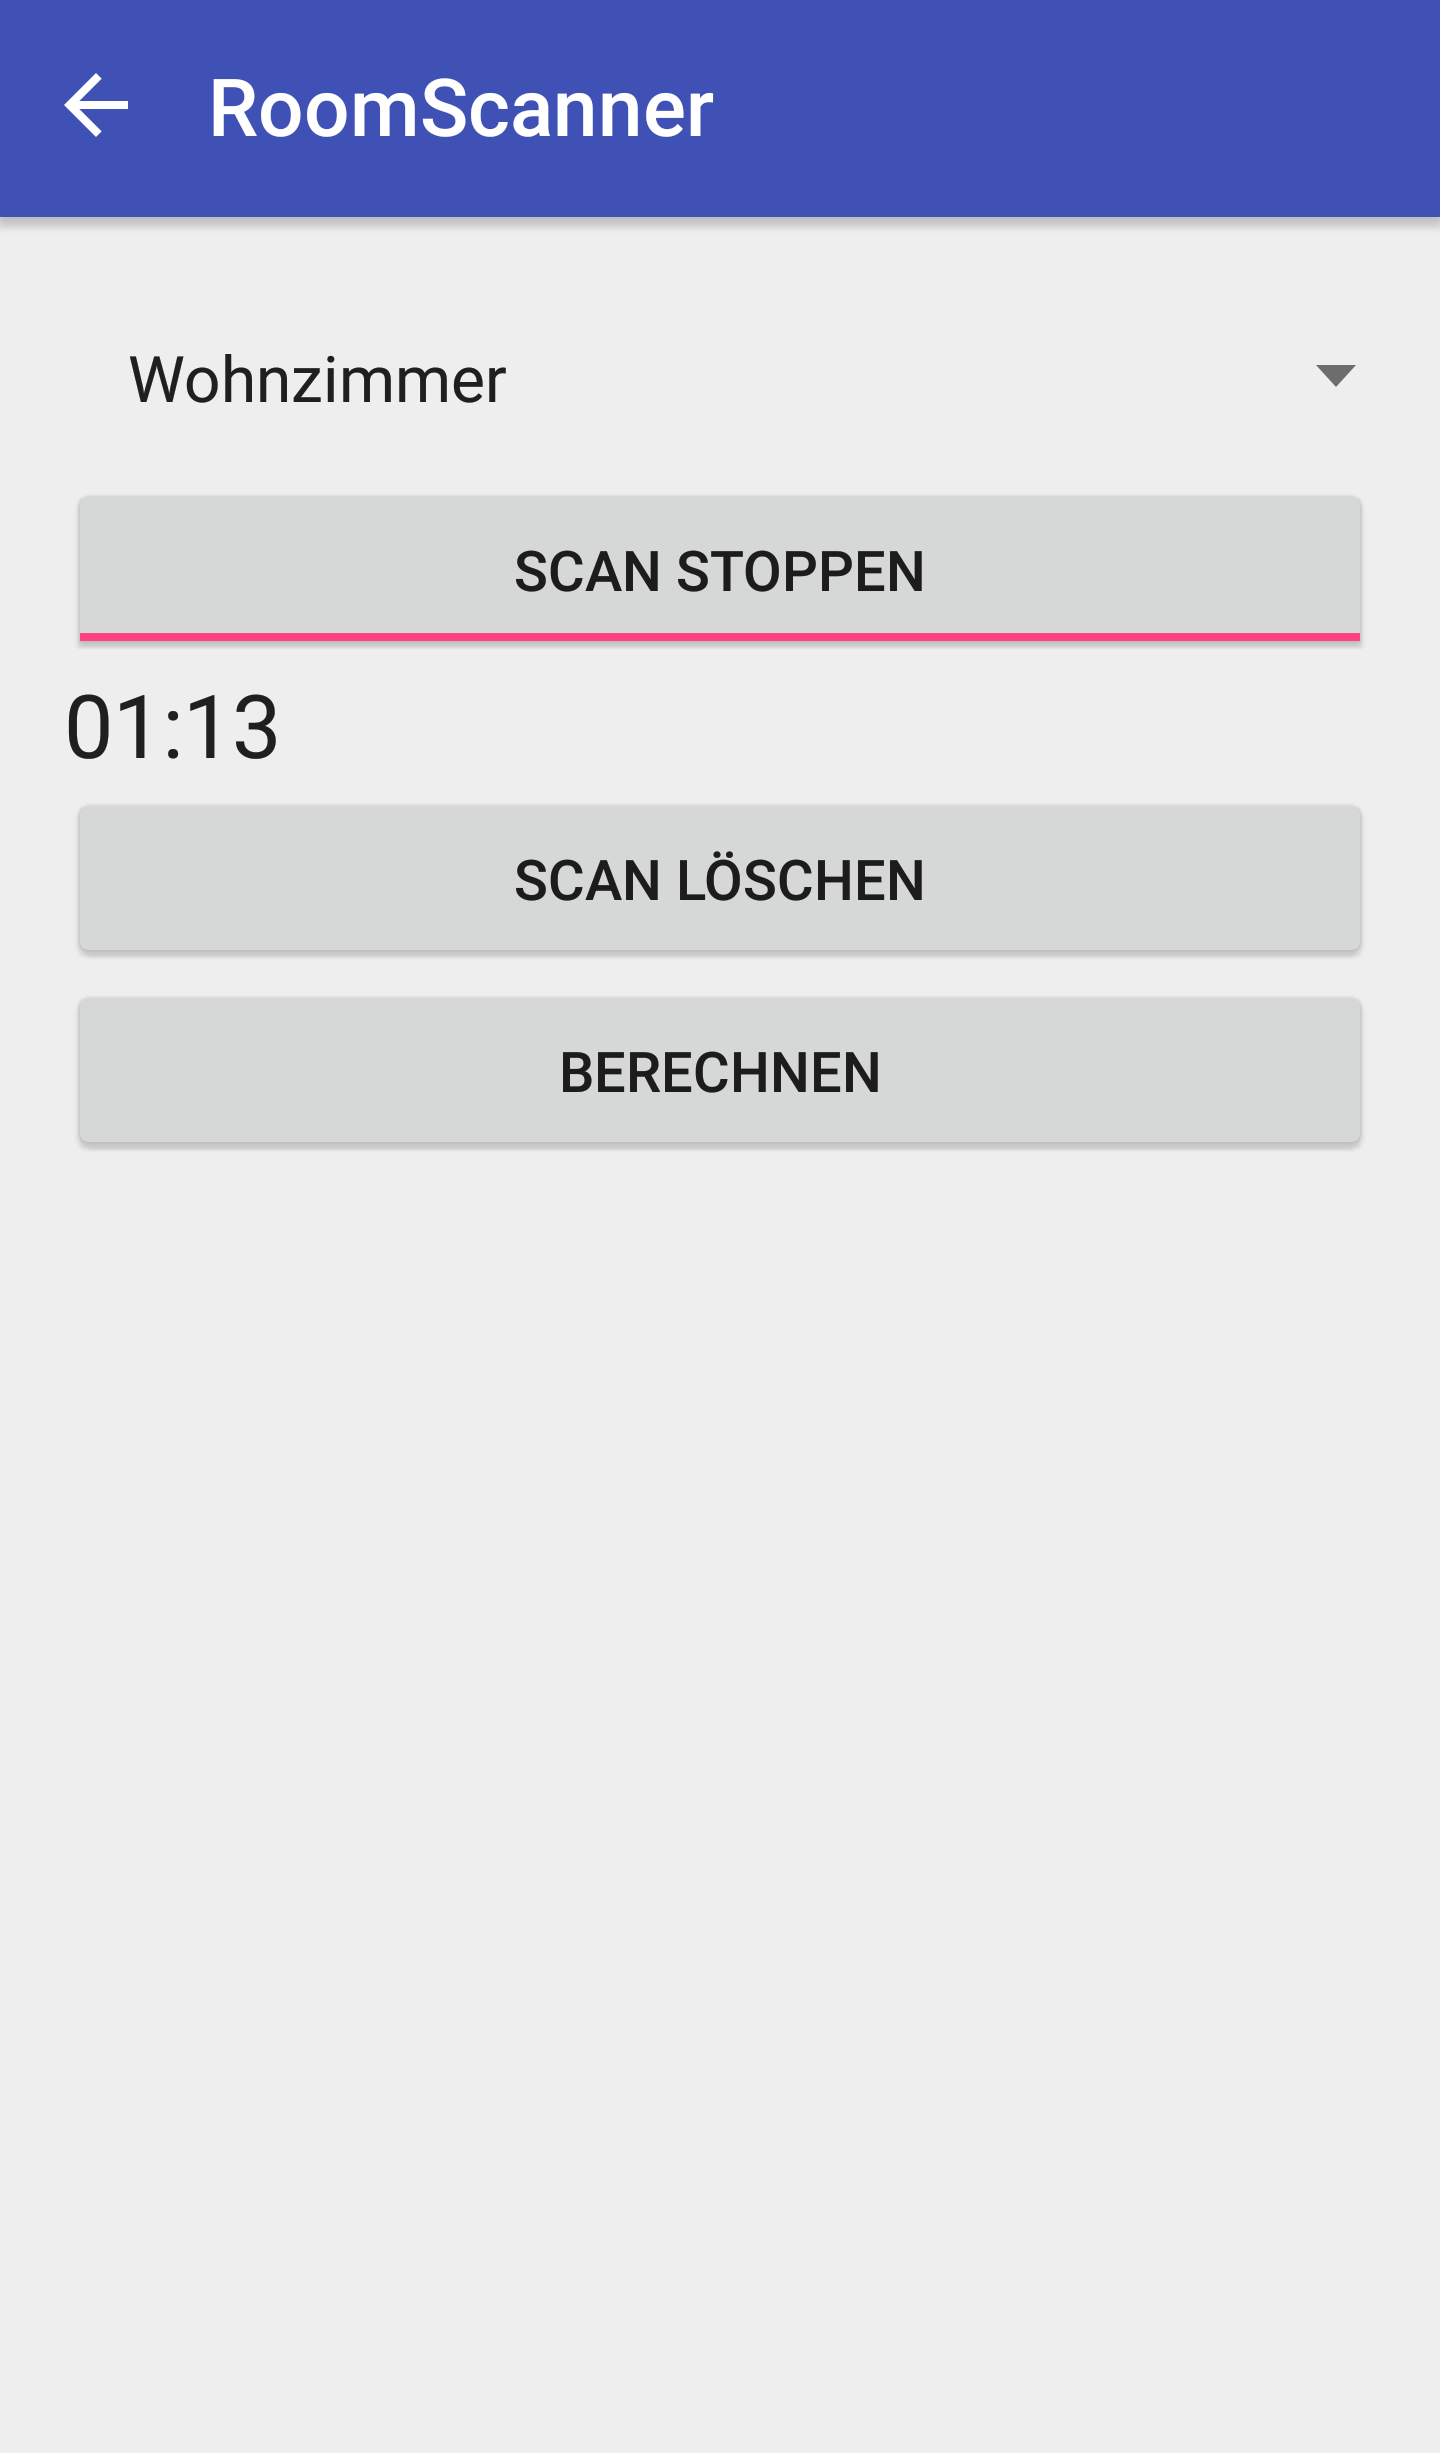
\includegraphics[width=0.4\linewidth]{../Bilder/ScreenshotPhoneRoomScanner}
\caption{Screenshot der Ansicht zum Vermessen von Räumen und Berechnen des Modells}
\label{fig:ScreenshotPhoneRoomScanner}
\end{figure}



